\documentclass[letterpaper, 10 pt, conference]{ieeeconf}  

\IEEEoverridecommandlockouts                              
\overrideIEEEmargins

\usepackage{graphicx}
\usepackage{float}
\usepackage{booktabs}
\usepackage[style=apa,sortcites=true,sorting=nyt,backend=biber]{biblatex}
\addbibresource{references.bib}
\title{\LARGE \bf
Optimizing the Bicycle Crossing between Vredenburg and Smakkelaarsveld
}


\author{\IEEEauthorblockN{Gijs van Dijk}
\IEEEauthorblockA{\\{Utrecht University}\\}}


\begin{document}

\maketitle

\thispagestyle{empty}
\pagestyle{empty}


\begin{abstract}

The bicycle crossing between Utrecht’s Vredenburg and Smakkelaarsveld is one of
the busiest in the Netherlands, with more than 30,000 daily crossings \parencite{utrect-2019}. This junction experiences a lot of congestion from the competing flows of bicycles, buses, and pedestrians. Bicycle paths in particular tend to get overcrowded. This research evaluates how potential infrastructure changes could improve throughput and reduce waiting times. We simulate bicycles, buses, and pedestrians and use queuing theory to model traffic flow and measure congestion through the utilization factor ($\rho$). The baseline simulation shows that bicycle lanes operate at more than double capacity with a mean ($\rho$) of 2.0491. Removal of a key bottleneck node significantly reduces this value to 1.4112. A 30\% decrease in bicycle volume yields a similar result. Combining both interventions lowers $\rho$ to 0.9892, indicating a stable and efficient crossing. These results show that both physical redesign and demand management are needed to reduce congestion at this intersection.

\end{abstract}


\section{INTRODUCTION}

The infrastructure in the city of Utrecht is facing more and more pressure. Recent results show that a large majority (89\%) of respondents find
the cycle paths in Utrecht busy, and nearly two-thirds (60\%) indicate they are
actively bothered by the crowds \parencite{winter-2020}. These values are higher than the Dutch national average \parencite{winter-2020}.

The Vredenburg-Smakkelaarsveld  has over 30,000 daily crossings \parencite{utrect-2019} and can get very congested. The junction connects the two main parts of the city, Utrecht Central Station and the city centre.
 
The current layout leads to a lot of congestion. This research combines a Python built agent simulation built on a graph network with analytical models
from queuing theory. Queueing theory models traffic as a stochastic service process driven by arrivals and departures. The utilization factor $\rho$ links demand, capacity, and delay. As $\rho$ approaches 1, queues grow quickly and waiting times rise. This relationship explains how congestion forms and why small increases in demand cause large delays \parencite{VANDAELE2000121}.


We use real-world data and simple statistical inference to evaluate performance of proposed infrastructure changes.

\section{Methodology}

\subsection{Graph Representation}

The crossing is modelled as a directed graph, $G = (V, E)$, which is a map of nodes and the paths that connect them (Figure 1). The nodes ($V$) are the key spatial points, such as entrances, exits, and waiting areas. The edges ($E$) are the one-way travel paths between these nodes. The style of the edge shows its type: straight lines are for bicycle paths, dashed lines are for buses, and dotted lines are for pedestrians. Each edge is assigned a weight that represents the physical distance to travel from one node to the next. This model allows us to analyse the real-world movement of traffic and identify potential bottlenecks in the system. For example, a bicycle might travel from the top right ($E$), to the bottom left ($G$), passing through node $H$.

\begin{figure}[H]
    \centering
    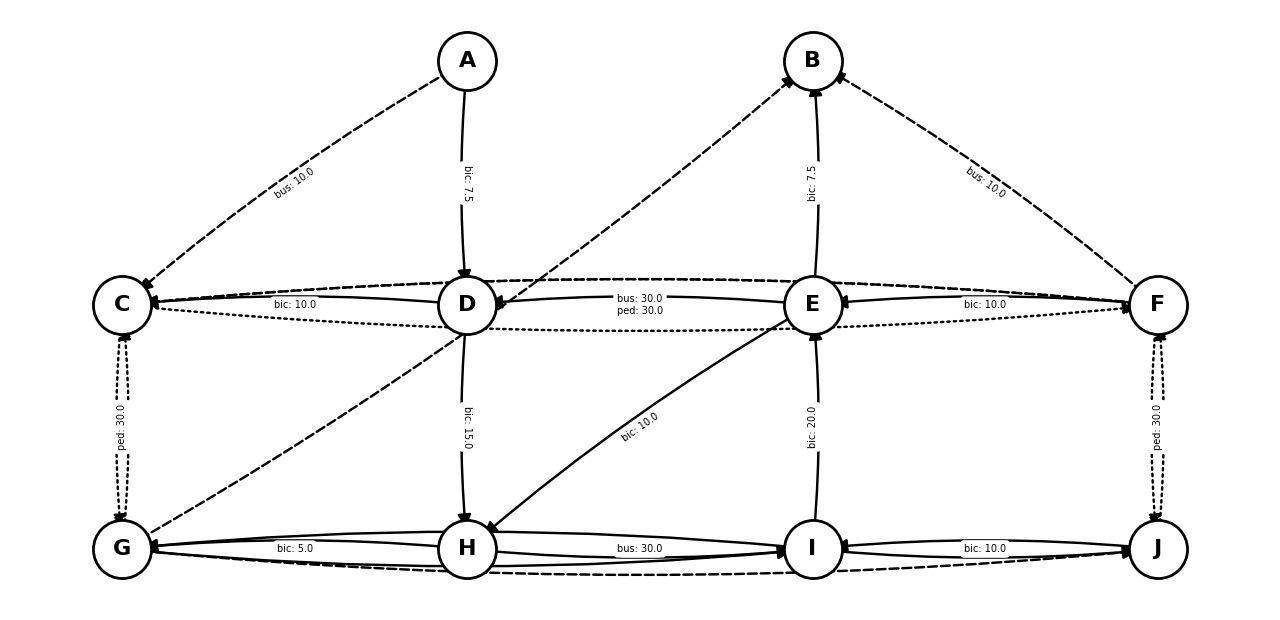
\includegraphics[width=\columnwidth]{graph_nolegend_v2.png}
    \caption{The graph representation of the Vredenburg network. Nodes (A-J) represent key spatial points. Edges are weighted by distance. Straight lines represent bicycles, dashed buses, and pedestrians dotted.}
    \label{fig:vredenburg_graph}
\end{figure}

\subsection{Simulation Framework}

A multi agent simulation is constructed in which each agent represents a cyclist, bus,
or pedestrian moving through the network.
Cyclists and buses follow measured arrival rates, while pedestrian movement is
modelled randomly.
By running the simulation described below for different configurations, e.g., different cycling route, less volume for a specific agent, the model can be used to measure throughput or performance in general under different design scenarios. The agents are spawned randomly, and randomly move towards any of the outer nodes that count as exits by following the possible path.

\subsection{Queuing Theory Model}
To analytically evaluate congestion, we apply queuing theory, focusing on the
utilization factor ($\rho$):

$$
    \rho = \frac{\lambda}{\mu}
$$
Where $\lambda$ is the arrival rate, i.e., how many cyclists, buses, or pedestrians arrive per tick. Each tick represents one second, thus for a 24 hour simulation we use ($60 \cdot 60 \cdot 24$) 86400 ticks. $\mu$ is the service rate, i.e., capacity per node per second. A higher $\rho$ indicates greater congestion and potential delay. For each proposed change, we compute a new utilization value ($\rho_{new}$) by running multiple samples and assess whether it represents a statistically significant improvement over the current state. This is done through statistical inference, comparing $\rho_{new}$ to the confidence interval of the baseline value.

\subsection{Configuration}
The simulation is configured to run for a total duration of 86,400 seconds, representing a full 24-hour cycle. A traffic light controller manages conflicting flows, operating on a 90-second total cycle time allocated sequentially to bicycles, pedestrians, and buses. A 10-second delay is set for the bus priority signal. 

The service capacity ($\mu$), representing the maximum number of agents a node can process per time unit, is set to 100 for pedestrians, 50 for bicycles, and 3 for buses. Pedestrians have the highest capacity due to their small size and ability to move in dense flows. Bicycles require more space, so their capacity is lower. Buses are large and take longer to move, which limits the number that can pass through a node at once. A systematic review of walking speeds finds that cross walk timing typically assumes 1.2 m/s for pedestrians \parencite{su16114813}, therefore agent speeds are set at 1.2 m/s for pedestrians.
We used 5.5 m/s for bicycles, and 8.33 m/s for buses, which corresponds to the 30 km/h maximum allowed speed in this area. The arrival (spawn) rates for bicycles and pedestrians are modelled using a bimodal distribution \parencite{park-2024} to simulate morning and evening commuter peaks, using the specified mean and standard deviation parameters in the configuration for each mode. A visual representation of this can be seen in figure 2. On daily average, one bus passes by per minute, per direction \parencite{studiobereikbaar2024}. We model this by letting buses arrive at a constant rate of 0.033 (2 buses / 60 seconds) agents per second in our model. Each agent type is assigned a specific list of permissible entry and exit nodes to define their valid routes through the network.

\begin{figure}[H]
    \centering
    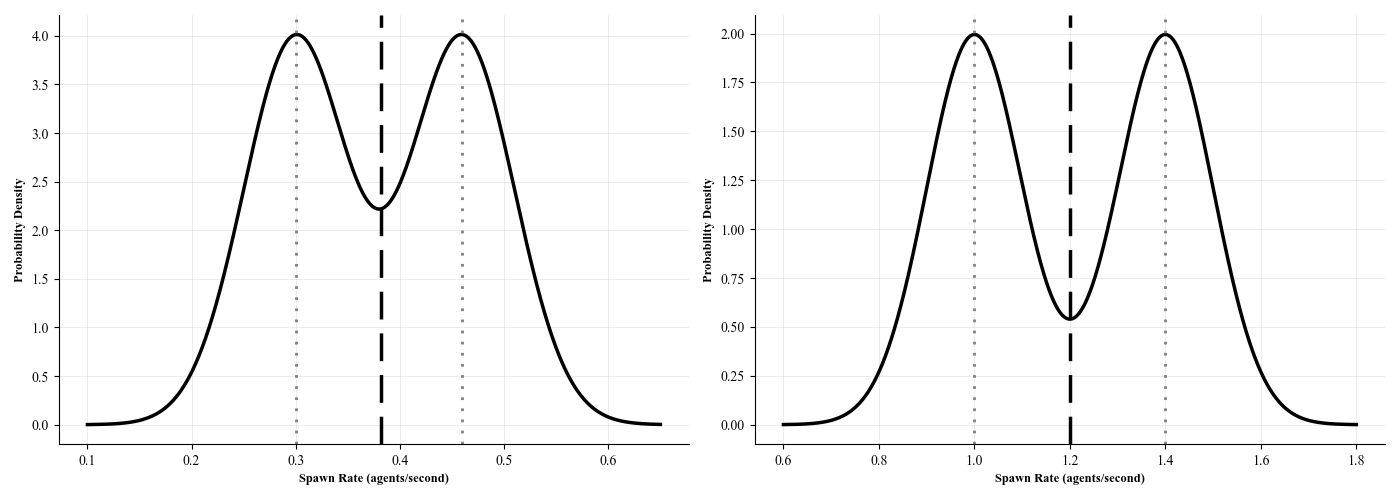
\includegraphics[width=\columnwidth]{bimodal_spawn.png}
    \caption{Visual representation of the bimodally distributed spawn rates for bicycle and pedestrian agents. Representing peak hours.}
    \label{fig:bimodal_graph}
\end{figure}

We use real-world data for the simulation model. The data is categorized by the mode of transport.

\subsubsection{Bicycles}
The daily average volume is 33,000 cyclists, with peak days reaching up to 47,000. Cyclist speeds are modelled with a speed of 5.5 meters per second (m/s). The arrival pattern of cyclists is known to be bimodally distributed, reflecting morning and evening peak hours \parencite{park-2024}. Furthermore, traffic flow is assumed to have an equal 50/50 split between inbound and outbound directions.

\subsubsection{Buses}
Key bus lines include 2, 3, 4, 5, 7, 8, 28, 55, 73, and 77. The combined frequency of these lines results in an average arrival rate of approximately one bus every two minutes at the crossing.

\subsubsection{Pedestrians}
For this research, which focuses on optimizing bicycle and bus flow, pedestrian movements are not our primary aim for research. Pedestrians can move only in simple paths purely regulated by traffic light intervals. High congestion of pedestrians is not as much of a problem as bicycles for example, since the crossing does not focus on pedestrians due to other possible routes available. Pedestrian agents are modelled using random arrival and movement patterns. 

\subsection{Statistical Validation}  
To establish the baseline performance, we first run our simulation \( n \) times for the \textit{current} system. From these \( n \) runs, we compute the sample mean utilization \({\rho}_{old} \) and the sample standard deviation \( s_{old} \). Because the number of simulation runs is limited (\( n \leq 30 \)) due to the computational costs, we use the \textit{t}-distribution instead of the normal (\textit{Z}) distribution.

\noindent The confidence interval (CI) for the true mean utilization of the old system (\( \rho_{old} \)) is therefore given by:  

\[
    CI_{old} = \rho_{old} \pm t^{*}_{\alpha/2, \, n-1} \cdot \left( \frac{s_{old}}{\sqrt{n}} \right)
\]

\noindent Here, \( {\rho}_{old} \) is the sample mean utilization of the current system, \( s_{old} \) is the sample standard deviation, and \( t_{\alpha/2, \, n-1} \) is the critical \textit{t}-value corresponding to a chosen confidence level with \( n - 1 \) degrees of freedom. 

\noindent The Null Hypothesis ($H_0)$ can be defined as 

$$H_0:\rho_{new}=\rho_{old}$$

and would conclude no significant difference. Subsequently, our Alternative Hypothesis ($H_a$) is 

$$H_a: \rho_{new} \neq \rho_{old}$$

\noindent We then perform \( n \) simulation runs for the new system to compute its sample mean utilization \( {\rho}_{new} \). If \( {\rho}_{new} \) falls outside the confidence interval \( CI_{old} \), we reject the null hypothesis \( H_0 \) and conclude that the difference between the two systems is statistically significant, i.e., the observed change in performance is unlikely to be due to random variation alone.


\section{Results}
In the baseline simulation of the Vredenburg-Smakkelaarsveld crossing, average
utilization ($\rho$) values were computed for pedestrians, buses, and bicycles over $n$ runs. 


\begin{table}[h]
	\caption{\textit{Descriptive Statistics for Baseline Utilization}}
	\label{tab:agent_performance}
		\begin{tabular}{lrrr}
			\toprule
			Metric & Pedestrians & Buses & Bicycles \\
			\midrule
			Mean ($\rho$) & \textbf{0.4316} & \textbf{0.3904} & \textbf{2.0491} \\
			Std Dev ($\sigma$) & 0.0016 & 0.0209 & 0.0016 \\
			95\% CI & [0.4296, 0.4335] & [0.3645, 0.4163] & [2.0472, 2.0511] \\
			\bottomrule
		\end{tabular}
\end{table}

For $n=30$ runs the results were that the bicycle lanes experienced the highest load with a mean $\rho=2.0491$ and a standard deviation $\sigma=0.0016$, compared to $\rho=0.4315$ $(\sigma=0.0016$) for pedestrians and $\rho=0.3904$ ($\sigma = 0.0209$) for buses (Table 1). These values suggest that the bicycle network operated well beyond its service capacity ($\rho>1$), implying a lot of congestion under the current baseline conditions. The 95\% confidence interval for the baseline was $[2.0472, 2.0511]$. 


The removal of bottleneck node $H$ resulted in a reduction of utilization. Applying a two-tailed t-test ($n=30$) to compare the before and after utilization confirms a statistically significant improvement for bicycles, as the new mean utilization factor ($\rho=1.4112$) lies outside the 95\% confidence interval ($[2.0472, 2.0511]$) of the baseline (Table 2)

\begin{table}[h]
	\caption{\textit{Descriptive Statistics for Utilization (No Node $H$)}}
	\label{tab:agent_performance}
		\begin{tabular}{lrrr}
			\toprule
			Metric & Pedestrians & Buses & Bicycles \\
			\midrule
			Mean ($\rho_{new}$) & \textbf{0.5399} & \textbf{0.3658} & \textbf{1.4112} \\
			Std Dev ($\sigma$) & 0.0046 & 0.0145 & 0.0048 \\
			95\% CI & \textbf{[0.5341, 0.5456]} & \textbf{[0.3478, 0.3838]} & \textbf{[1.4053, 1.4171]} \\
			\bottomrule
		\end{tabular}
\end{table}

%% add something about to which value bicycles were decreased %%
Since the $\rho_{new}$ mean still implies high congestion ($\rho>1>1.4112$) we do not have a valid solution yet.
Besides infrastructure, policy and traffic control could be a solution to the congestion. Since the utilization factor is calculated with the arrival rate ($\lambda$) in the numerator, a lower arrival rate would mean less utilization, and thus less congestion. Therefore, we modelled the effect of 30\% less bicycle traffic. Solely decreasing the number of bicycles per day by 30\% reduced the utilization to a similar level as removing node $H$ ($\rho=1.4353, \sigma=0.0007$). This measurement was ran with $n=5$ samples. Ultimately, we modelled the reduction of bicycles in combination with removing node $H$. This resulted in a mean $\rho$ of 0.9892 with a standard deviation ($\sigma$) of 0.0054. Since this utilization is smaller than 1 ($\rho\leq0.9892<1$), we can conclude that there is less usage than total capacity.

\section{Discussion}
The results from the baseline simulation provide a measure of the congestion at the crossing. The key finding is that the mean bicycle utilization ($\rho=2.0491$) runs at double its capacity. In comparison, pedestrian ($\rho=0.4316$) and bus ($\rho=0.3904$) flows operate well within their capacity limits. This shows that the junctions primary failure is its inability to process the bicycle traffic volume.

Our first intervention, removing bottleneck node $H$, caused significant improvement. The new mean bicycle utilization $\rho_{new}=1.4112$ (Table 2) falls well outside the 95\% confidence interval of the baseline $[2.0472, 2.0511]$. This result confirms that this node ($H$) is a major contributor to the inefficiency of the junction. The experiment modelling a 30\% reduction in bicycle traffic ($\lambda$) yielded a similar result in utilization factor ($\rho=1.4353$). This suggests that managing the amount of traffic is as important as the physical infrastructure. This could practically be achieved by developing new, more attractive, and parallel bicycle routes. The Vredenburg-Smakkelaarsveld path is the main connector between the station and the city centre. Creating multiple alternative paths would distribute this demand, preventing all cyclists from taking this single junction.

Additionally, the problem can be addressed by increasing the service rate ($\mu$). In our model, the service rate is directly proportional to the number of agents a node can process. This capacity is determined by the width of the bicycle paths and the size of the waiting areas. Widening these paths would directly increase $\mu$, allowing more cyclists to pass be second. This would lower the utilization $\rho$ without needing to reduce the total number of cyclists. 

The combined strategy of removing node $H$ and reducing bicycles by 30\% resulted in a mean utilization of $\rho=0.9892$ which is below the 1.0 threshold. This indicates that the system can, on average, service all arriving cyclists

The study has limitations. The model, while effective for analysing flows, simplifies the pedestrian movements as random. It also did not capture small behaviours such as cyclists overtaking or buses being delayed. The bimodal spawn rates are also a simple approximation of more complex daily patterns. Real world conditions may present even higher peaks. 

The small standard deviations and narrow confidence intervals result from the deterministic setup of the model. Spawn rates and movements are modelled randomly, which allows for noise. 

\section{Conclusion}
This research used agent simulation and queuing theory to analyse the Vredenburg-Smakkelaarsveld crossing. The baseline model confirmed that bicycle traffic operates at more than double the junctions capacity, resulting in severe congestion. 

The junction's diagonal top right to bottom left pass from node $E$ to node $H$ seems obsolete when you take a look at the graph (Figure 1). Since bicycles are still allowed to move from the right side of the junction to the left by taking the horizontal route (i.e., from $E$ to $D$).

We evaluated that removing node $H$, which represents the diagonal pass for the bicycles, offered a significant improvement in utilization. This change alone, however, was insufficient to bring the system below its capacity limit. Similarly, a 30\% reduction in the volume of bicycles was also insufficient. A stable and efficient solution was only achieved when both strategies were combined. The removal of node H paired with a 30\% reduction in bicycle traffic lowered the system's utilization factor to ( $\rho=0.9892$). This is the only scenario modelled that represents a functionally stable crossing.

\section{Future Research}
Traffic follows more sophisticated paths than modelled in this paper,  so future research could follow up on this paper by building in these algorithms. \parencite{NI2024100022}.

The model is not entirely deterministic, but the small variances ($\sigma$) and confidence intervals show that more noise could be modelled in.

Dynamic bicycle paths using pressure plates or sensors are getting more popular, and could be a focus for future research. By actively measuring congestion using sensors and taking according action the throughput could be improved \parencite{puts-2018}

Further collaboration with the municipality and transport agencies (U-OV for Utrecht) may also enable
field experiments to validate results and test the impact of proposed design changes.

%% might change symbols %%

\newpage

\printbibliography
\end{document}
